\documentclass[12pt]{report}
\usepackage[top=1in, bottom=1in, left=1in, right=1in, a4paper]{geometry}

 \ifx\pdftexversion\undefined
 \usepackage[dvips]{graphicx}
 \else
 
 \usepackage[pdftex]{graphicx}
 \DeclareGraphicsRule{*}{mps}{*}{}
 \fi
%\usepackage{tabularx,colortbl}
\usepackage{url}
\usepackage{chapterbib}
\usepackage{hyperref}
\usepackage{tabularx}
%\usepackage{tikz}
%\usepackage{pgfplots}
%\usepgfplotslibrary{groupplots} 
%\usepackage{pgf, pgfarrows, pgfnodes}
\usepackage{lscape}
\usepackage{longtable}
\usepackage{float}
\usepackage{url}
\usepackage{multicol}
\usepackage{color}
\usepackage{float}
\usepackage{paralist}
%\usepackage[none]{hyphenat}
\renewcommand{\bibname}{References}
\usepackage{listings}
\setcounter{secnumdepth}{4}
\setcounter{tocdepth}{4}
\definecolor{codegreen}{rgb}{0,0.6,0}
\definecolor{codegray}{rgb}{0.5,0.5,0.5}
\definecolor{codepurple}{rgb}{0.58,0,0.82}
\definecolor{backcolour}{rgb}{0.95,0.95,0.92}
\lstdefinestyle{mystyle}{
    backgroundcolor=\color{backcolour},   
    commentstyle=\color{codegreen},
    keywordstyle=\color{magenta},
    numberstyle=\tiny\color{codegray},
    stringstyle=\color{codepurple},
    basicstyle=\footnotesize,
    breakatwhitespace=false,         
    breaklines=true,                 
    captionpos=b,                    
    keepspaces=true,                 
    numbers=left,                    
    numbersep=5pt,                  
    showspaces=false,                
    showstringspaces=false,
    showtabs=false,                  
    tabsize=2
}
 
\lstset{style=mystyle}



\begin{document}

\begin{titlepage}
 \begin{center}
\LARGE
\textbf{Cloud based IT Infra with Central Identity} \\
%\vfill
%\large
%\textbf{\{ Project reboot \}}\\
\vfill
\textbf{Phase II -- Project Report }\\
\vfill
\Large
\underline{\textbf{Project Guide }} \\ 
\large
\underline{} \\
T. Chandra Shekar \\
\small
Dept. of CSE -- RGUKT Nuzvid \\
\small
\url{chandra.indra@gmail.com}
\vfill

\Large
\textbf{\underline{ Project Team } } \\
\underline{} \\
\large
\begin{tabular}{l  l}
T. Aneesh Kumar & N090247  \\
P. Nageswarao  & N091030  \\
P. Anesh  & N090977  \\
P. Jyothi Ram & N090990  \\
K. Naresh Chowdary  & N090331  \\
N. Venkata Sateesh  & N090935  \\
M. Sanyasi Rao & N090891 
\end{tabular}

\vfill



\includegraphics[width=3.5cm]{rgukt_logo.jpg} 
\Large
\underline{} \\
\underline{} \\
\normalsize
\textbf{Dept. of Computer Science and Engg. } \\
\textbf{R.G.U.K.T. - Nuzvid } \\
\textbf{Krishna Dt. - Andrha Pradesh - 521202}


\normalsize
\vfill
%\begin{multicols}{2}
%\begin{flushleft}
%\textbf{Start Date} : Sep 2014 \\
%\end{flushleft}
%
%
%\begin{flushright}
%\textbf{End Date} : Jan 2015 \\
%\end{flushright}
%\end{multicols}

\textbf{Sep 2014 -- Dec 2014 }

\end{center}
\end{titlepage}

% \pagebreak \thispagestyle{empty} \textcolor{white}{text} \pagebreak
 
\chapter*{Abstract}
\setcounter{page}{1}
\pagenumbering{roman}
\normalsize
\hspace{0.5cm} The main objective of ``Cloud based IT Infra with Central Identity'' Phase II is provide the implementation to our objectives. \newline

Implementing the Web based central identity, network based central identity, achieve the combination and deploy all these in the private cloud \newline

%\pagebreak \thispagestyle{empty} \textcolor{white}{text} \pagebreak

\setcounter{page}{2}
\pagenumbering{roman}
\tableofcontents
\listoffigures
\listoftables
\pagebreak \thispagestyle{empty} \pagebreak

 
\setcounter{page}{1}
\pagenumbering{arabic}


\chapter{Introduction}

\section{Introduction}
	``Cloud Based IT Infra with Central Identity'' is a complete solution, based on private cloud to enhance and effiecient utilization the IT Infrastructure of an emerging Universities and Organizations with Central Identity for all its users to access its services.\newline

	It is going to be developed in 3 phases 
	\begin{itemize}
		\item \textit{Private cloud} 
		\item \textit{Deploying Network Services} 
		\item \textit{Central Identity}
	\end{itemize}
	
\subsection{Private Cloud}

	Private Cloud establishment is targeted for hardware resource pooling, providing high computational and scalable virtual machines for deploying network based applications (smtp, proxy, ftp), web application and Network storage.
	
\subsection{Deploying Network Services}

	Configuration of Uniform hardware experience over the complete university includes single sign on on every device, configuration of mail servers etc.
	
\subsection{Central Identity}

	Essential part that combines normal network services(proxy, mail, etc.) and organizational web \& native applications. In addtion to that this central identity is available to thrid party developers as API with dynamic based role user authentication protocols.	
	
\chapter{Phase I Work}

	As part of Phase I, we have done literature survey and anlyzed feasability of the several components
	
\section{Components}

	\begin{itemize}
		\item Central Identity
		\begin{itemize}
			\item Single Sign-On with REST API
			\item Identity Management
			\item Dynamic Role Based Access Control
		\end{itemize}
		\item Network Based Central Identity
		\begin{itemize}
			\item LDAP Servers
			\item NFS Servers
		\end{itemize}
		\item Cloud Computing
		\begin{itemize}
			\item 	Cloud Characterstics
			\item Service Models 
			\item Deployment Models 
		\end{itemize}		 
		\item Private Clouds 
		\begin{itemize}
		 	\item Introduction 
			\item Open Source Tools 
		\end{itemize}			

	\end{itemize}

\chapter{Phase II Work}

	As part of Phase II, we have tried to implement some of the above mention components 

\section{Components}

	\begin{itemize}
		\item Web based Signle Sign On
		\begin{itemize}
			\item OAuth Provider 
			\item University Users Profiles 
			\item REST API 
			\item Support of assigin roles to users with their permission set
			\item Testing oauth client library in PHP using php-curl
		\end{itemize}
		\item Network Components
		\begin{itemize}
			\item LDAP Server
			\item NFS Server
			\item Haproxy
			\item GlusterFS
			\item XtreemFS
			%\item DOS Attacks
		\end{itemize}
		\item Private Infrastructure Cloud
		\begin{itemize}
			\item Openstack Architecture
			\item Installation
			\item Virtual Machines
		\end{itemize}		 			

	\end{itemize}
\chapter{Network Single Sign-On}
\section{Introduction}
	
	Single sign-on (SSO) is a session/user authentication process that permits a user to enter one name and password in order to access multiple applications. The process authenticates the user for all the applications they have been given rights to and eliminates further prompts when they switch applications during a particular session.\\
	\underline{} \newline
	\textbf{Components Used:} 
	\begin{itemize}
	\item LDAP Server
	\item phpLdapAdmin
	\end{itemize}

\section{LDAP Server}

	LDAP, or Lightweight Directory Access Protocol, is a protocol for managing related information from a centralized location through the use of a file and directory hierarchy. It functions in a similar way to a relational database in certain ways, and can be used to organize and store any kind of information. LDAP is commonly used for centralized authentication.

\subsection{Installation and Configuration}
	The OpenLDAP server is in Ubuntu's default repositories under the package "slapd". We have to install some additional utilities in order to use it in full pledged way.
	
	\begin{itemize}
	\item sudo apt-get \textbf{update}
	\item sudo apt-get install \textbf{slapd ldap-utils}
	\end{itemize}

	After the installation is complete, we actually need to reconfigure the LDAP package by the following
	\begin{itemize}
	\item sudo \textbf{dpkg-reconfigure slapd}
	\end{itemize}
	
	\pagebreak
		By following below steps we have to configure the LDAP
	\begin{itemize}
		\item Omit OpenLDAP server configuration? \textbf{No}
		\item DNS domain name? \textbf{reboot.org}
		\item Organization name? \textbf{reboot}
		\item Administrator password? \textbf{Password}
		\item Database backend to use? \textbf{HDB}
		\item Remove the database when slapd is purged? \textbf{No}
		\item Move old database? \textbf{Yes}
		\item Allow LDAPv2 protocol? \textbf{No}
	\end{itemize}
\section{phpLDAPadmin}	
	
	It’s a web-based LDAP client. It provides easy, anywhere-accessible, multi-language administration for LDAP server. By this configuration and monitor of LDAP Server will be done in an easy way. \\
\underline{} \newline
Its hierarchical tree-viewer and advanced search functionality make it intuitive to browse and administer your LDAP directory. Since it is a web application, this LDAP browser works on many platforms, making your LDAP server easily manageable from any location.
\subsection{Installation and Configuration}
	\begin{itemize}
	\item sudo apt-get install \textbf{phpldapadmin}
	\end{itemize}
	
	After the installation is complete configuration will be done by making following changes in the
config.php file of phpLDAPadmin.
	\begin{itemize}
	\item sudo nano \textbf{/etc/phpldapadmin/config.php}
	\end{itemize}

	\lstinputlisting[language=PHP,caption=PHP Config file]{conf.php}

\subsection{Web Interface of phpLDAPadmin:}
	%\subsubsection{Authentication:}

		\begin{figure}[H]
		\begin{center}
		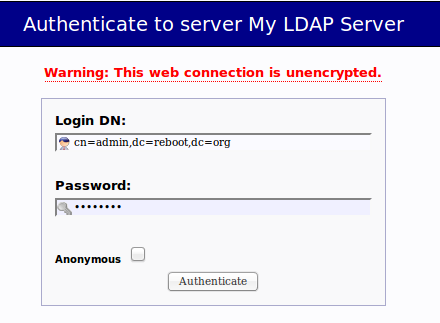
\includegraphics[width=8cm,height=6cm]{Screens/LdapServerLogin.png}
		\caption{phpLDAP \label{fig: phpLDAP Image}}
		\end{center}
		\end{figure}

	%\subsubsection{Server’s sidebar with complete information:}
		\begin{figure}[H]
		\begin{center}
		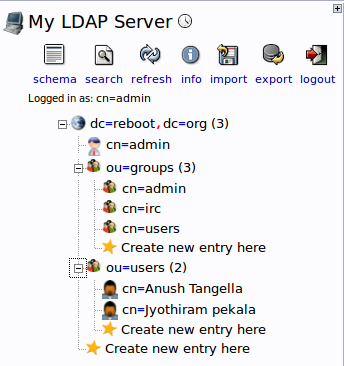
\includegraphics[width=8cm,height=8cm]{Screens/serversidebar.png}
		\caption{Complete category of LdapServer \label{fig: Complete category of LdapServer}}
		\end{center}
		\end{figure}
	
	%\subsubsection{User Creation in LDAP server:}
		\begin{figure}[H]
		\begin{center}
		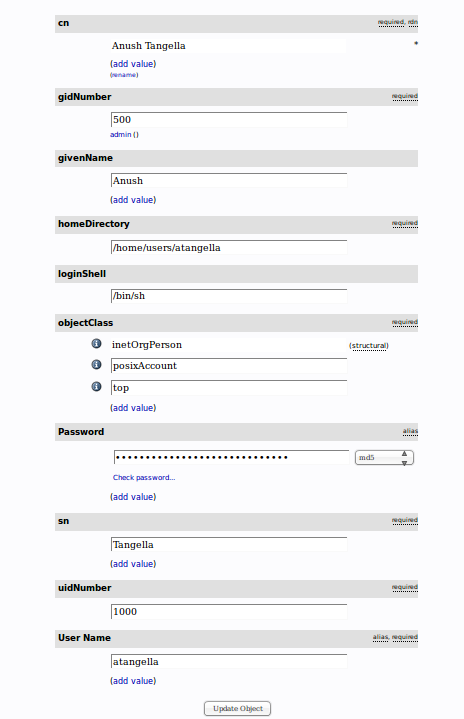
\includegraphics[width=10cm,height=15cm]{Screens/UserCreation.png}
		\caption{User Creation \label{fig: User Creation}}
		\end{center}
		\end{figure}

	%\subsubsection{Creating Group:}	
		\begin{figure}[H]
		\begin{center}
		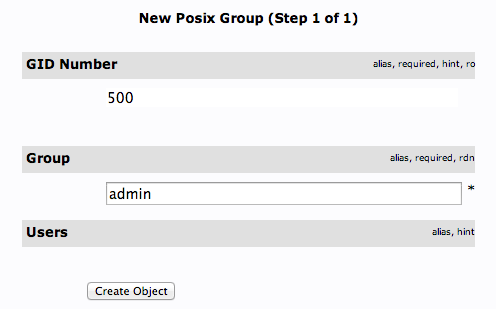
\includegraphics[width=8cm,height=6cm]{Screens/admin_group.png}
		\caption{Group Creation \label{fig: Group Creation}}
		\end{center}
		\end{figure}		
		
	%\subsubsection{Adding user to Group:}
		\begin{figure}[H]
		\begin{center}
		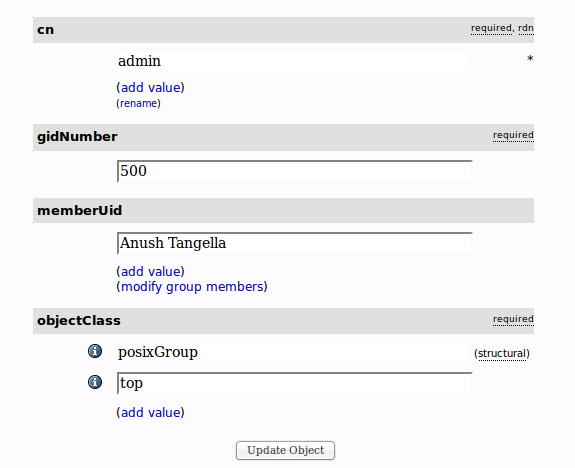
\includegraphics[width=10cm,height=8cm]{Screens/AddUsertoGroup.png}
		\caption{Adding User to Group \label{fig: Adding User to Group}}
		\end{center}
		\end{figure}
		
	%\subsubsection{Groups complete information:}
		\begin{figure}[H]
		\begin{center}
		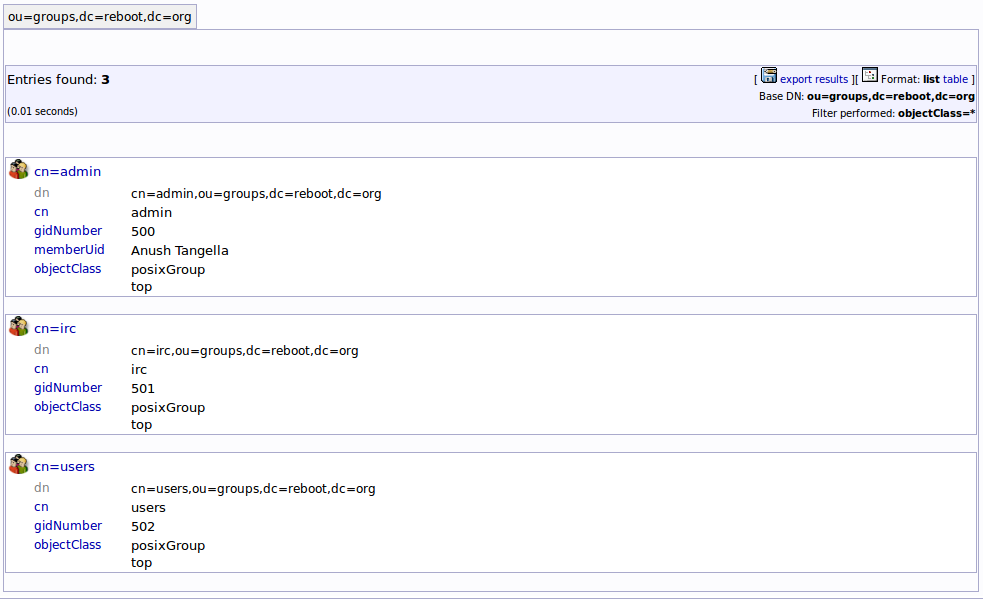
\includegraphics[width=17cm,height=10cm]{Screens/Groupsinfo.png}
		\caption{Groups information \label{fig:Groups information}}
		\end{center}
		\end{figure}
		
\section{LDAP Client:}		
	LDAP, or Lightweight Directory Access Protocol, is one way of keeping authentication information in a single centralized location. We need another droplet to act as the client machine.
	\subsection{Installation and Configuration:}
		On the client machine, we need to install a few packages to make authentication function correctly with an LDAP server.	
		\begin{itemize}
		\item sudo apt-get install \textbf{libpam-ldap nscd}
		\end{itemize}		 
By following these below steps we need to configure the LDAP Client
		\begin{itemize}
		\item LDAP server Uniform Resource Identifier: \textbf{ldap://10.4.34.47/} from \textbf{``ldapi:///''}		
		\end{itemize}

		Distinguished name of the search base:
		This should match our values in LDAP server's /etc/phpldapadmin/config.php file.
		\begin{itemize}
		\item We have to replace " 'server','base',array " within the file to \textbf{``dc=reboot,dc=org''}
		\item LDAP version to use:\textbf{ 3}
		\item Make local root Database admin: \textbf{Yes}
		\item Does the LDAP database require login? \textbf{No}
	 	\item LDAP account for root:
		 	\begin{itemize}
	 		\item This should also match with our values in your \textbf{/etc/phpldapadmin/config.php}
			\item Search for: \textbf{`` ` login ' , ` bind\_id ' '' } within the file
			\item Our example was \textbf{``cn=admin,dc=reboot,dc=org''}
		 	\end{itemize}
		\end{itemize}
		LDAP root account password: \textbf{Our-LDAP-root-password}
		\\
		\linebreak
		If made a mistake and need to change a value, we can go through the menu again by issuing this command:
		\begin{itemize}
		\item sudo \textbf{dpkg-reconfigure ldap-auth-config}
		\end{itemize}
		
		To configure client we adjust a few files that they can look to our LDAP server for authentication information.
		First, we have to edit the /etc/nsswitch.conf file. This will allow us to specify that the LDAP credentials should be modified when users issue authentication change commands
		\begin{itemize}
		\item sudo nano \textbf{/etc/nsswitch.conf}
		\end{itemize}
		\pagebreak
		The three lines we are interested in are the "passwd", "group", and "shadow" definitions. 
		Modify them to look like this:
		\lstinputlisting[language=sh,caption=Config file]{nsswitch.conf}
		
		We have to add the values to our PAM configuration.
		
		PAM, or Pluggable Authentication Modules, is a system that connects applications that can provide authentication to applications that require authentication.
		When we installed and configured our LDAP PAM module, most of the needed information was added to the configuration files and we need to edit below file.
		\begin{itemize}
		\item sudo nano \textbf{/etc/pam.d/common-session}
		\item sudo nano \textbf{/etc/pam.d/login}
		\item sudo nano \textbf{/etc/pam.d/lightdm}
		\end{itemize}
		
	We have to add the below piece of code to each of the above PAM configuration files
		\begin{itemize}
		\item session required \textbf{pam\_mkhomedir.so skel=/etc/skel umask=0022x}
		\end{itemize}
		
		The above will create a home directory on the client machine when an LDAP user logs in who does not have a home directory.
		We have to restart a service for these changes to be implemented:
		\begin{itemize}
		\item sudo \textbf{/etc/init.d/nscd restart}		
		\end{itemize}
		
		\subsection{Log In as an LDAP User:}
		We have now configured our client machine enough to be able to log in as one of our LDAP users. This user does not have to exist on the client machine.
		In order to connect to LDAP Client, we have to ssh into that particular machine.
		\begin{itemize}
		\item ssh \textbf{atangella@10.4.34.45}
		\end{itemize}


\chapter{Private Infrastructure Cloud}
To support this central identity both the network and web network central identity we want to go for the private cloud deployment it includes creating the Private Infrastructure Cloud with openstack and creating Virtual Machines for instaling these services and assign them the IP address.

\section{Openstack Architecture}
Openstack is a cloud operating system that provides the 3 main services for the Infrastructure clouds namely Stoage, Compute, Networking and some other components are can be added later as addons
\underline{} \newline
\begin{figure}[H]
	\begin{center}
	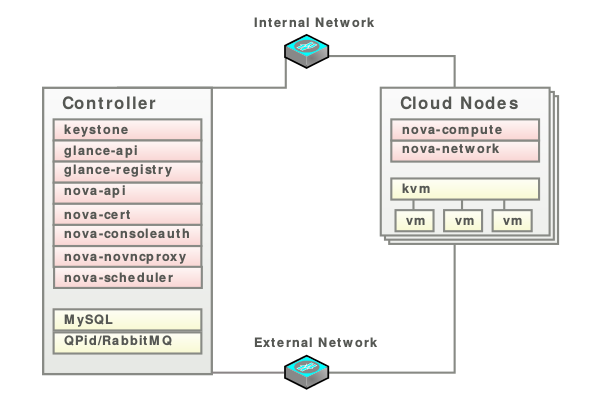
\includegraphics[width=11cm,height=8cm]{./openstack_1.png}
	\caption{ Openstack Architecture.\label{fig:Openstack Architecture }}
	\end{center}
\end{figure}

\section{Installation}

Installing openstack includes component wise installation namely NTP, MySQL, Rabbitmq-Server, Keystone, Nova, Cinder, Glance, Neutron
\subsection{NTP}
\# apt-get install ntp
\subsection{MySQL}
\# apt-get install mysql-server
\subsection{Rabbitmq-server}
\# apt-get install rabbitmq-server
\subsection{Keystone}
\# apt-get install keystone
\subsection{Glance}
\# apt-get install glance python-glanceclient
\subsection{Nova}
\# apt-get install nova-api nova-cert nova-conductor nova-consoleauth nova-novncproxy nova-scheduler python-novaclient
\subsection{Neutron}
\# apt-get install neutron-server neutron-plugin-ml2
\pagebreak
\section{Virtual Machines}
This Virtual Machines are created from the resource pool after successfull installation openstack
\begin{figure}[H]
	\begin{center}
	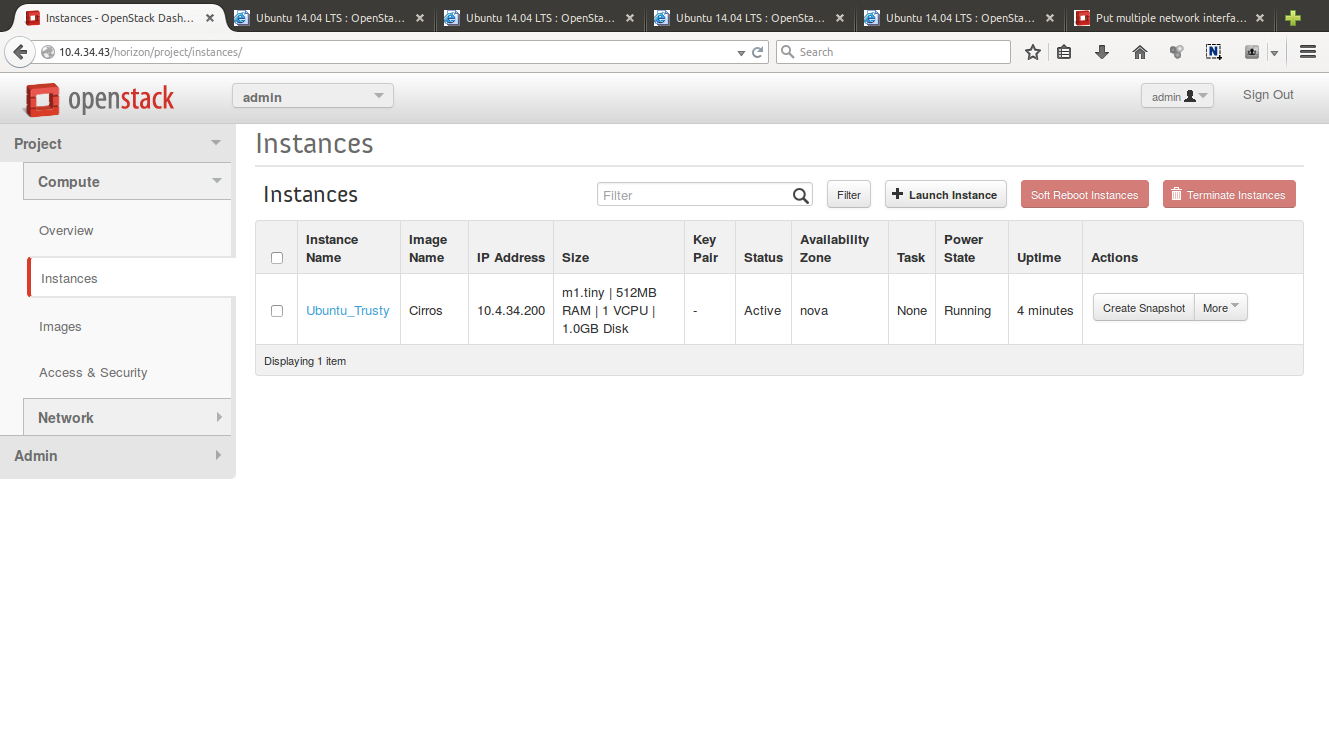
\includegraphics[width=12cm,height=8cm]{./openstack_2.png}
	\caption{ Openstack Virtual Machines.\label{fig:Openstack Virtual Machines }}
	\end{center}
\end{figure}
\begin{figure}[H]
	\begin{center}
	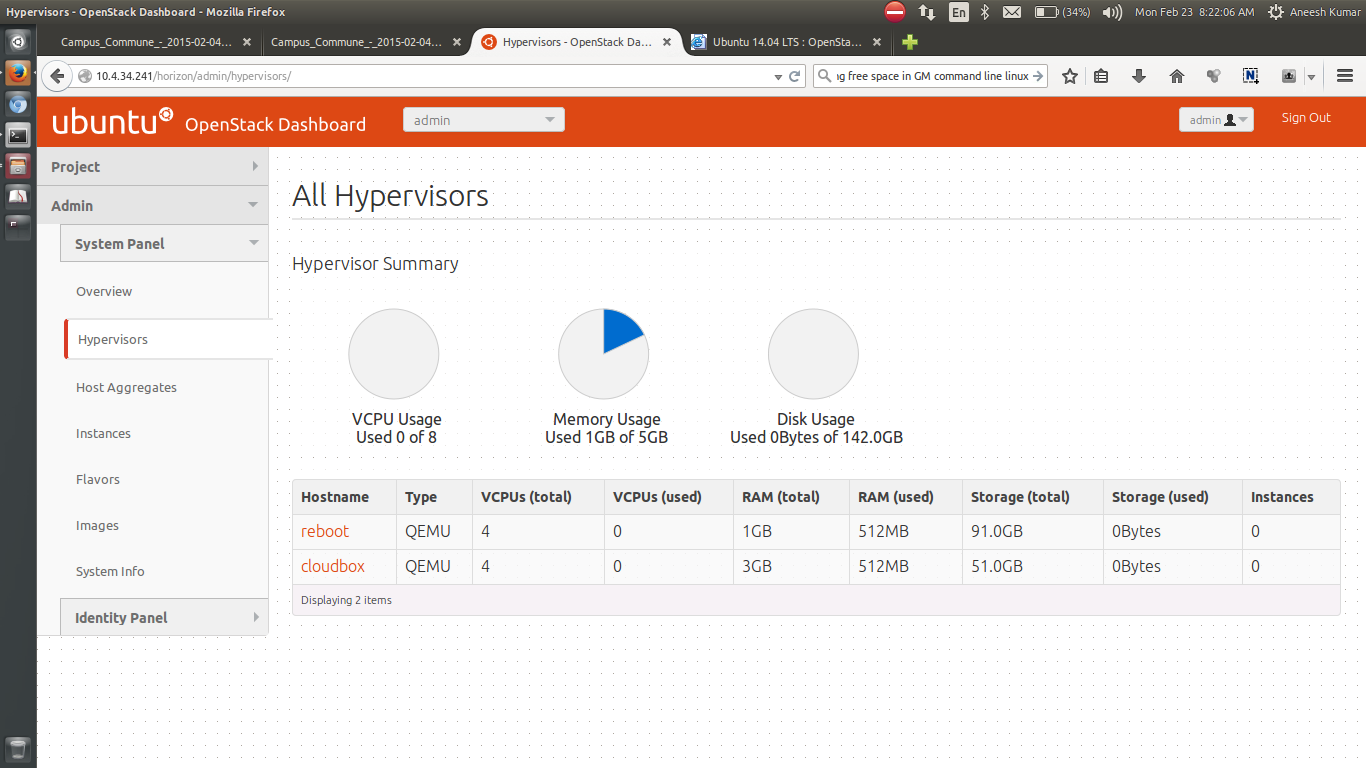
\includegraphics[width=12cm,height=8cm]{./openstack_3.png}
	\caption{ Openstack Resource Pool.\label{fig:Openstack Resource Pool }}
	\end{center}
\end{figure}
\chapter{Conclusion \& Future Work}
\section{Conclusion} 
We tried GlusterFS for replication among systems, but it’s not working if any one of the system fails. Then we found that XtreemFS works well in distributed system and provides fault tolerant solution. \newline
\underline{} \newline
We developed network based sign on using LDAP and web based single sign on along with REST API using Oauth 2.0 and Django. We tried to create private cloud using openstack but lot of errors came because of proxy based internet and low configured PCs.

\section{Future Work}
We would like to combine Network single sign-on with Web based single sign on along with XtreemFS and HAProxy. Creating virtual machines and Private cloud is not possible with the available systems. But if we could provide systems with enough configuration, sure we can create better sophisticated solution

\chapter{References}

\end{document}